\section{Memento}

O padrão Memento é útil para implementar funcionalidades 
de \textit{checkpoint} ou de "desfazer", já que permite 
armazenar e restaurar o estado interno de um objeto 
sem que ele seja exposto. Dessa forma, o encapsulamento 
não é violado, mesmo que o estado seja armazenado externamente.

Isso é alcançado através de uma classe Memento que armazena os 
atributos de um objeto que precisa ser salvo. A responsabilidade 
de criar a cópia, assim como a de recuperar os atributos copiados, 
é do próprio objeto. A estrutura do padrão pode ser vista 
na figura \ref{memento_struct}.

\begin{figure}[htb]
	\caption{\label{memento_struct}Estrutura do Memento}
	\begin{center}
	    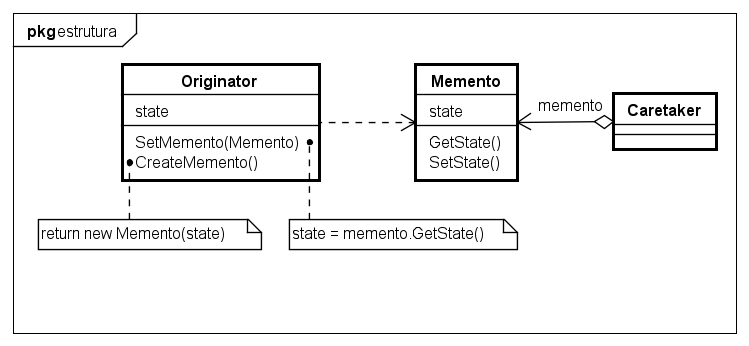
\includegraphics[scale=0.5]{5_padroes-contexto-funcional/5.3_comportamentais/5.3.06_memento/memento_estrutura.png}
	\end{center}
\end{figure}

\subsection*{Exemplo Orientado a Objetos}

Como exemplo, pode ser considerado um editor de texto que 
suporta operações de desfazer. O editor pode armazenar um 
\textit{snapshot} de seu estado atual em uma classe que 
armazena o histórico de alterações. Dessa forma, quando a 
operação de desfazer for executada, basta que o 
\textit{snapshot} mais recente seja recuperado pelo histórico 
e restaurado no editor. A figura \ref{memento_exemplo} demonstra 
esse exemplo, enquanto o código \ref{oomemento} demonstra a 
implementação.

\begin{figure}[htb]
	\caption{\label{memento_exemplo}Exemplo de Memento}
	\begin{center}
	    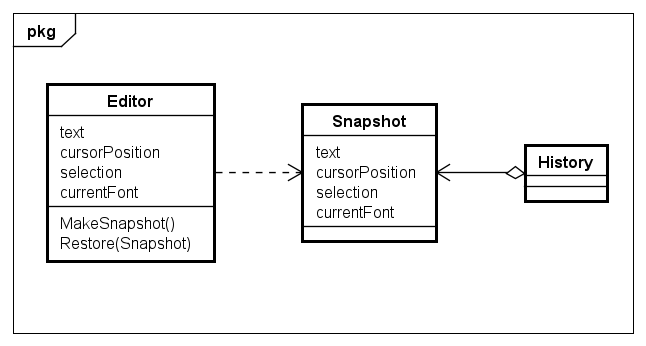
\includegraphics[scale=0.5]{5_padroes-contexto-funcional/5.3_comportamentais/5.3.06_memento/memento_exemplo.png}
	\end{center}
\end{figure}

\begin{lstlisting}[caption={Memento Orientação a Objetos},label=oomemento]

class Editor(private var text:String,
             private var cursorPosition : Position,
             private var selection : (Position, Position),
             private var currentFont : String) {

  def MakeSnapshot() : Snapshot = {
    new Snapshot(text, cursorPosition, selection, currentFont)
  }

  def RestoreSnapshot(snapshot: Snapshot) : Unit = {
    this.text = snapshot.text
    this.cursorPosition = snapshot.cursorPosition
    this.selection = snapshot.selection
    this.currentFont = snapshot.currentFont
  }
}

class Snapshot (val text : String,
                val cursorPosition : Position,
                val selection : (Position, Position),
                val currentFont : String)
                
class History {
  private var snapshots : List[Snapshot] = List.empty

  def AddSnapshot(snapshot: Snapshot) : Unit = {
    snapshots = snapshots :+ snapshot
  }

  def GetSnapshot() : Snapshot = {
    val snapshot = snapshots.head
    snapshots = snapshots.tail
    snapshot
  }
}

\end{lstlisting}

\subsection*{Contexto Funcional}

Como os dados são imutáveis, não é necessário 
preocupar-se com funções externas modificando o 
estado do valor que se deseja guardar. Dessa forma, 
armazenar os \textit{checkpoints} em uma coleção, como 
uma lista, é suficiente para resolver o problema 
proposto pelo padrão.

O código \ref{fpmemento} apresenta duas funções, 
CreateSnapshot na linha 2 e RestoreSnapshot na linha 
5. A primeira recebe como parâmetro o valor que 
deve ser salvo e a lista de valores já salvos. 
O retorno é apenas a lista de valores atualizada. 
Já a segunda recebe como parâmetro a lista de 
valores salvos e retorna uma tupla cujo 
primeiro elemento é o novo valor, restaurado 
a partir da lista, e o segundo valor é a 
lista atualizada com o valor recuperado 
removido.

\begin{lstlisting}[caption={Memento Funcional},label=fpmemento]

def CreateSnapshot(editor : Editor, snapshots : List[Editor]) : List[Editor] =
  editor :: snapshots

def RestoreSnapshot(snapshots : List[Editor]) : (Editor, List[Editor]) =
  (snapshots.head, snapshots.tail)

\end{lstlisting}